\documentclass{article}
\usepackage{amsthm,amsmath,amsfonts,lipsum}
\usepackage[T1]{fontenc}
\usepackage{beramono}
\usepackage{listings}
\usepackage{fontawesome5}
\usepackage{adjustbox}
\usepackage{mathabx}
\usepackage{thmtools}
\usepackage{import}
\usepackage{graphicx}
\usepackage{setspace}
\usepackage{geometry}
\usepackage{physics}
\usepackage{float}
\usepackage[english]{babel}
\usepackage{framed}
\usepackage[dvipsnames]{xcolor}
\usepackage{tcolorbox}
\usepackage{fullpage}
\usepackage{indentfirst}
\usepackage{lastpage}
\usepackage{enumerate}
\usepackage{fancyhdr}
\usepackage{mathrsfs}
\usepackage{xcolor}
\usepackage{listings}
\usepackage{hyperref}
\usepackage[utf8]{inputenc}
\usepackage{booktabs}
\usepackage{enumitem}
\usepackage{animate}
\usepackage{tikz}

\newcommand{\incfig}[1]{%
    \def\svgwidth{\columnwidth}
    \import{./figures/}{#1.pdf_tex}
}

\newcommand{\sincfig}[1]{%
    \def\svgwidth{0.7\columnwidth}
    \import{./figures/}{#1.pdf_tex}
}
\newcommand{\hs} {
\hspace{1cm}
}

\newcommand{\vs}{
\vspace{1cm}
}
\setlength{\fboxsep}{10pt}

\colorlet{LightGray}{White!90!Periwinkle}
\colorlet{LightOrange}{Orange!15}
\colorlet{LightGreen}{Green!15}

\newcommand{\HRule}[1]{\rule{\linewidth}{#1}}

\declaretheorem[style=thmsty,numberwithin=section]{theorem}
\tcolorboxenvironment{theorem}{colback=LightGray}

\declaretheoremstyle[name=Proposition,]{prosty}
\declaretheorem[style=prosty,numberlike=theorem]{proposition}
\tcolorboxenvironment{proposition}{colback=LightOrange}

\declaretheoremstyle[name=Principle,]{prcpsty}
\declaretheorem[style=prcpsty,numberlike=theorem]{principle}
\tcolorboxenvironment{principle}{colback=LightGreen}

\setstretch{1.2}
\geometry{
  textheight=9in,
  textwidth=5.5in,
  top=1in,
  headheight=12pt,
  headsep=25pt,
  footskip=30pt
}

\definecolor{codepurple}{RGB}{138, 43, 226}
\definecolor{codeblue}{RGB}{0, 0, 255}
\definecolor{codegray}{RGB}{128, 128, 128}
\definecolor{codegreen}{RGB}{0, 128, 0}
\definecolor{customgray}{RGB}{243, 243, 243}

\lstset{
    language=C,
    basicstyle=\ttfamily\tiny, % Imposta il carattere del codice a \small
    keywordstyle=\color{codepurple},
    stringstyle=\color{codeblue},
    commentstyle=\color{codegray}\itshape,
    numberstyle=\tiny\color{codegray},
    backgroundcolor=\color{white},
    tabsize=4,
    showspaces=false,
    showstringspaces=false,
    breaklines=true,
}

\tcbuselibrary{skins}
\definecolor{boxTitle}{HTML}{fff79a}
\definecolor{boxBackground}{HTML}{fffce0}
\definecolor{boxFrame}{HTML}{f1e2b8}

\tcbset{my box/.style={
    enhanced, fonttitle=\bfseries,
    colback=boxBackground, colframe=boxFrame,
    coltitle=black, colbacktitle=boxTitle,
    attach boxed title to top left={xshift=0.3cm,
                                    yshift*=-\tcboxedtitleheight/2},
    boxed title style={
      before upper=\hspace*{0.5cm}, % reserve space for the image
      overlay={
       \node at ([xshift=0.5cm]frame.west)
         {\includegraphics[scale=0.015]{./figures/dodecahedron2.png}};
      }
    }
  }
}
\newtcolorbox{mybox}[1][]{my box, #1}
\newlength{\overwritelength}
\newlength{\minimumoverwritelength}
\setlength{\minimumoverwritelength}{1cm}

%---------------------Red Box---------------------------
\newcommand{\rbox}[3][red]{%
  \settowidth{\overwritelength}{$#2$}%
  \ifdim\overwritelength<\minimumoverwritelength%
    \setlength{\overwritelength}{\minimumoverwritelength}\fi%
  \stackrel
    {%
      \begin{minipage}{\overwritelength}%
        \color{#1}\centering\small #3\\%
        \rule{1pt}{9pt}%
      \end{minipage}}
    {\colorbox{#1!50}{\color{black}$\displaystyle#2$}}}

% ------------------------------------------------------------------------------

\begin{document}

% ------------------------------------------------------------------------------
% Cover Page and ToC
% ------------------------------------------------------------------------------

\title{ \normalsize \textsc{}
  \\ [2.0cm]
  \HRule{1.5pt} \\
  \LARGE \textbf{\uppercase{Calcolo Numerico}
  \HRule{2.0pt} \\ [0.6cm] \LARGE{Guida all'orale} \vspace*{10\baselineskip}}
}
\date{}
\author{\textbf{Author} \\ 
  Marco Omicini (TüT) \\
  Università degli studi del Molise \\
Luglio 2023}

\maketitle
\newpage

\tableofcontents
\newpage

% ------------------------------------------------------------------------------

\section{1-cfu}

\begin{theorem}
  This is a theorem.
\end{theorem}

\begin{proposition}
  This is a proposition.
\end{proposition}

\begin{principle}
  This is a principle.
\end{principle}

% Maybe I need to add one more part: Examples.
% set style and colour later.

\subsection{pictures}

\subsection{citation}

this is a citation\cite{eg}.

\newpage

\subsection{problemi ben posti (hadamard)}
un problema matematico si può esprimere nella forma 
\begin{equation}
  f(x,d)=0 \label{eq:problema matematico}
\end{equation}
dove $x$ e $d$ possono essere qualsiasi cosa, come matrici, vettori, numeri reali o anche funzioni. in questa sede, stiamo considerando un problema matematico astratto, non legato a situazioni specifiche. \\
il problema $f(x,d)=0$ è \textbf{ben posto} se e solo se esiste una sola soluzione $x$, e tale soluzione dipende in modo continuo dai dati.\\
se almeno una delle tre condizioni non è verificata, il problema sarà \textbf{mal posto}, e non avrebbe senso affrontarlo da un punto di vista numerico e richiederebbe una sua riformulazione.

\subsection{problemi ben condizionati}
un problema si dice \textbf{ben condizionato} se piccole perturbazioni sui dati producono piccole perturbazioni sui risultati. consideriamo il problema perturbato $f(x+\delta x, d+\delta d)$. allora deve valere quanto segue:
\begin{equation}
  \exists k_0=k(d)\text{ tale che }\forall\delta d:d+\delta d\in d,\|\delta x\|\leq k_0\|\delta d\|.
\end{equation} 

dove $\norm{\cdot}$ rappresenta la norma euclidea o una qualsiasi altra norma matematica appropriata. in altre parole, se la perturbazione sui dati è proporzionale alla perturbazione sui risultati, allora il problema è ben condizionato.\\
al contrario, un problema \textbf{mal condizionato} è caratterizzato da un'elevata sensibilità alle perturbazioni sui dati, il che lo rende più difficile da risolvere correttamente.\\ 
\begin{tcolorbox}[colback=white,colframe=black,title=nota]
  $k_0$ è una costante detta indice di condizionamento\\
  $d$ è l'insieme dei dati ammissibili. \\
  $\forall \delta d : \delta d + d \in d$ ci assicura che il dato perturbato $\delta d + d$ sia ancora un dato ammissibile per il problema
\end{tcolorbox} 

\subsection{indice di condizionamento}
definiamo, per il problema matematico \eqref{eq:problema matematico}, l'indice di condizionamento, ossia il valore che ci indica quanto sono sensibili i risultati rispetto a una perturbazione sui dati. 
\begin{equation}
  k_{rel}(d)=\sup\left\{\frac{\|\delta x\|/\|x\|}{\|\delta d\|/\|d\|},\delta d\neq0,d+\delta d\in d\right\}. 
\end{equation} \\ \\ \\
nel caso in cui $d = 0$ o $x=0$ ha più senso introdurre \textit{l'indice di condizionamento assoluto}:
\begin{equation}
  k_{abs}(d)=\sup\left\{\frac{\|\delta x\|}{\|\delta d\|},\delta d\neq0,d+\delta d\in d\right\}. 
\end{equation}
come possiamo immaginare ormai, un $k_0$ grande indicherà che il problema è molto sensibile a perturbazioni sui dati, di conseguenza più $k_0$ sarà "grande" più il problema sarà mal condizionato\\ \\
la proprietà di condizionamento del problema prescinde il metodo numerico (aka l'algoritmo) che andremo poi ad utilizzare per risolverlo.\\ 
difatti come già preannunciato prima, un problema mal posto, ossia un problema tale per cui esistono più soluzioni (o non ne esiste nessuna) \\ 
oppure un problema tale per cui i risultati non dipendono in maniera continua dai dati (mal condizionato)
non merita di essere proprio affrontato, perché ha dei disagi profondi che l'algoritmo non sarà in grado di risolvere. \\
un problema di questo tipo, quindi, necessiterà una riformulazione tale per cui venga rispettata la proprietà di ben posizione. \\

\begin{tcolorbox}[colback=white,colframe=black,title=nota]
  potrebbe creare un po di confusione, almeno per me è così, il fatto che la definizione di mal condizionamento è un pò ambigua.\\ 
  infatti il termine "grande" lascia un po a desiderare visto che "grande" è una grandezza non definita.\\ 
  per chiarire diremo che al crescere di $k_0$ crescerà il mal condizionamento del problema.\\ 
  se $k_0 = \infty$ allora siamo sicuri che il problema è mal condizionato (e quindi anche mal posto visto che non vale piu la dipendenza continua dei risultati dai dati) 
\end{tcolorbox} 

\subsection{stabilità di un algoritmo} 
supponendo che il probelma sia ben posto allora un metodo numerico consisterà, in generale, nel costruire una serie di probelmi approssimanti 
\begin{equation}
  f_n(x_n,d_n)=0,\quad n\geq1 
\end{equation} 
con la speranza che per $n \to \infty$ si verifichi che $x_n \to x$ ossia che la soluzione approssimante tenda alla soluzione effettiva.\\ 
per essere più precisi vorremmo che si verifichi quanto segue:
\begin{equation}
  f_n(x_n,d_n)-f(x,d)\to0 \text{ per }n\to\infty 
\end{equation}
ossia che la successione di problemi approssimanti converga al problema effettivo.\newpage
\textbf{definizione:} un metodo numerico si dirà \textbf{stabile} se 
\begin{enumerate}
  \item l'errore si mantiene limitato e non cresce all'aumentare del numero delle operazioni \item ogni sotto problema $f_n(x_n,d_n)$ è ben posto
\end{enumerate}
un algoritmo che non rispetta anche una sola di queste proprietà si dirà \textbf{instabile}

\subsection{rappresentazione floating point}
se vi chiedessi di eseguire questa motliplicazione, quanto tempo ci mettereste?
\begin{equation}
  0,00000000034 \times 
  1343400000000
  \label{eq:motliplicazione base 10 senza notazione scientifica}
\end{equation}
sarebbe una spina nel fianco da fare come operazione vero? \\ 
un modo per semplificarci di molto la vita è togliere quella virgola, e segnarci in qualche modo la sua posizone.\\ 
possiamo quindi rappresentare il numero $0,00000000034$ come $34 * 10^{-12}$ e il numero $1343400000000$ come $13434 * 10^{8}$ \\
ora l'operazione che prima ci sembrava complicata da fare è decisamente piu semplice. infatti basta fare $34 * 13434 = 456756$ e aggiungere i due esponenti $-12 + 8 = -4$  ottenendo in definitiva $$
456757 * 10^{-4} = 4,56756 
$$
questa viene detta \textit{notazione scientifica} e porta con se un concetto importante che abbiamo appena visto:\\
\begin{proposition}
la posizione della virgola la decide l'esponente. questo ci permette di far fluttuare la virgola dove ci pare \textit{(floating point)}
\end{proposition}
più formalmente diremo: \\ \\
un numero reale $x$ può essere rappresentato come
\begin{equation}
  m \times b^{esp} \hspace{1cm} m \in \mathbb{r}, \ esp \in \mathbb{n}, 
\end{equation}
$m$ viene detta \textbf{mantissa}, $b$ viene detta \textbf{base} mentre $esp$ viene detto \textbf{esponente} o \textbf{caratteristica} \\
quindi fissata una base, ogni numero reale $x$ può essere rappresentato tramite la coppia $(m,esp)$ \\
il  numero $0$ per convenzione viene rappresentato tramite la coppia $(0,0)$ \\
ciò che abbiamo visto poco fà può essere applicato anche nei calcolatori, difatti basta solo ragionare in termini di $0$ e $1$\\ \\
ottimo! facciamo un esempio e rappresentiamo il numero 12,3. \\ 
la prima cosa da fare è convertirlo in binario. 
per fare ciò dobbiamo spezzare il numero, quello che c'è prima della virgola e quello che c'è dopo. 
risolviamo quindi il $12$ e ricaviamo la sua rappresentazione binaria. per farlo usiamo la nota tecnica della divisione (dividere sistematicamente il numero fino a reggiungere lo zero, memorizzando il resto per ogni divisione): 
\begin{equation}
  \begin{array}{rcl}
  12 / 2 & = & 6 \quad (0) \\  
  6 / 2 & = & 3 \quad(0) \\  
  3 / 2 & = & 1\quad (1) \\  
  1 / 2 & = & 0\quad (1) \\  
  \end{array}
  \label{eq:conversione decimale binario 1 }
\end{equation}
ora prendiamo il numero \textit{dall'alto verso il basso} ottenendo così che $12_{10} = 1100_{2}$ \\ 
occupiamoci adesso dell'altro pezzo, ossia $0,3$. \\ 
per convertire questo numero in binario possiamo usare la tecnica della motliplicazione (moltiplicare sistematicamente il numero memorizzando ogni volta se abbiamo raggiunto o meno un intero): 

\begin{equation}
\begin{aligned}
\begin{array}{rcl}
0,3 \times 2 & = & 0,6 \quad (0) \\
0,6 \times 2 & = & 1,2 \quad (1) \\
0,2 \times 2 & = & 0,4 \quad (0) \\
0,4 \times 2 & = & 0,8 \quad (0) \\
0,8 \times 2 & = & 1,6 \quad (1) \\
0,6 \times 2 & = & \cdots \
\end{array}
\end{aligned}
\left.
\begin{aligned}
 \\
 \\
 \\
\end{aligned}
\right \} \text{pattern}
\label{eq:conversione floatig binario 1}
\end{equation}
notiamo immediatamente il pattern ricorsivo, quindi non ha senso continuare a fare operazioni. \\
benissimo, abbiamo i due pezzetti che ci interessano $12,3 = 1100,0100110011001\dots$ 
ora usiamo la notazione scientifica per indicare la posizione della virgola. allora sappiamo che dovrà fare tre salti a sinistra per sparire, quindi l'esponente è pari a $4$. \\  
possiamo quindi rappresentare questo numero nella forma $m * b^{esp}$ (normalizzazione)\\ 
$$ m = 110001001100110011001100\dots, \hspace{1cm} esp = 100, \hs b = 2$$ \\
bello vero?\\
facciamo adesso un passo avanti e contestualizziamo questo ragionamento. \\ 
la rappresentazione binaria ci servirà in scenari reali, e quindi la giocata che abbiamo appena fatto (concedere alla mantissa un numero infinito di cifre) non è stata molto onesta. \\ 
prendiamo dunque il nostro pennello e ritocchiamo quanto abbiamo appena fatto.\\ \\
prima di tutto dobbiamo trovare un modo per regalare un bit alla mantissa così da poterne indicare facilmente il segno. 
quindi d'ora in poi il bit piu singificativo (quello più a sinistra) della mantissa indicherà il segno ($0 =$ positivo, $1=$ negativo)\\ 
per quanto rigurada l'esponente possiamo fare un gioco diverso. invece di regalare un bit aggiuntivo anche a lui, possiamo usare una tecnica chiamata \textit{bias dell'esponente}.\\ 
questa tecnica consiste nel sommare all'esponente $127$ e rappresentare quel valore. la conversione avverrà allo stesso modo, ossia sottraendo $127$ all'esponente \\ 
per quanto riguarda lo spazio da dedicare a mantissa ed esponente possiamo seguire i seguenti due approcci.
\newpage
\begin{figure}
    \centering
    \begin{tcolorbox}[arc=4pt]
      \centering
      \incfig{singolaprecisione} \\
    \end{tcolorbox}
    \vs
    \begin{tcolorbox}[arc=4pt]
      \centering
      \incfig{doppiaprecisione} 
    \end{tcolorbox}
\end{figure}

consideriamo che, nell'esempio del numero $2,3$ se decidessimo di dare alla mantissa $5$ bit otterremmo un'appossimazione pari a $2,25$\\ 
questo ci fa capire che più cifre diamo meglio è! \\ 
basta infatti salire a $8$ e otteniamo un'approssimazione di $2,29$ circa. \\ 
ovviamente, non potremmo mai ottenere $2,3$, perche per farlo dovremmo rappresentare tutte le infinite cifre della mantissa, ed è proprio qui che si nascondono i disagi della rappresentazione numerica.   

 
\subsection{insieme dei numeri macchina} 
Bene prociediamo a definire bene questo insime di numeri. \\
Sia $f(b,s,l,u)$ l'insieme dei numeri macchina, dove $b$ è la nostra base, $s$ rappresenta la grandezza consentita per la mantissa, mentre $l$ e $u$ sono rispettivamente il range inferiore e superiore dell'esponente tale per cui $l  \leqslant esp  \leqslant u$ \\ \\
se un numero dovesse essere troppo piccolo allora sappiamo che l'esponente, negativo, è più piccolo di quanto il nostro caclolatore può offrire, ossia è \textit{minore} di $l$  di conseguenza o viene lanciato un errore oppure si approssima quel valore a zero.\\ 
questa situazione viene detta \textbf{\textit{underflow}}\\ \\ 
se invece un numero dovesse avere, nella sua rappresentazione $x = m \times b^{esp}$ un esponente \textit{maggiore} di $u$ allora avremmo a che fare con la situazione opposta, ossa il numero è troppo grande per essere memorizzato, e di conseguenza si fa un'approssimazione dello stesso.\\
questo scenario viene detto \textbf{\textit{overflow}}\\ \\ 

\begin{proposition}
  l'insieme dei numeri macchina non consiste di punti equispaziati. 
\end{proposition}
questo perché ci sono più numeri binari possibili con un bit significativo rispetto a quelli che ci sono con due bit significativi e man mano che ci allontaniamo dallo $0$ il numero di bit usabili diminuisce, facendo diminuire anche il numero di numeri rappresentabili. \\
difatti l'insieme dei numeri macchina è piu denso vicino lo zero e meno denso man mano che ci si allontana 
 
\subsection{operazioni di arrotondamento}
se un numero $x$ rappresentato nella forma $m \times b^{esp}$ con $l \leqslant esp \leqslant u$ dovesse avere una mantissa con un numero di cifre superiorio a quello consentito, quindi $m > s$ allora si dovrà effettuare un arrotondamento per quel numero $x$ \\ 
per fare questo si aggiunge $\frac{1 }{2 }b^{-s}$ e si tronca all's-esima cifra. \\
intuitivamente significa che si aggiunge $0.5$ in ultima posizione e poi si tronca, questo non è altro che il noto arrotondamento per eccesso o per difetto.  
\subsection{errore di arrotondamento}

per quanto riguarda l'errore che l'arrotondamento porta con se, il suo calcolo è molto semplice e faremo distinzione tra due tipi di errore: l'errore relativo e quello assoluto \\ 
dato $x = m \times b^{esp}$ una soluzione e $\bar{x} = \bar{m} \times b^{esp}$ una sua approssimazione, possiamo quindi definire \\ \\
\large \textbf{errore assoluto}\\
\normalsize questo errore è la differenza tra la soluzione effettiva e quella approssimata e  rappresenta l'intervallo entro il quale il valore vero della grandezza si trova.\\ 
\begin{equation}
  \abs{x-\bar{x}} 
  \label{eq:errore assoluto}
\end{equation}
\large \textbf{errore relativo} \\
\normalsize l'errore assoluto ci da un'indicazione dell'intervallo entro in quale ci aspettiamo ragionevolmente che si trovi il valore vero della grandezza osservata però non descrive un quadro completo della situazione.\\
infatti mentre un errore di un centimetro su una distanza di un chilometro indicherebbe una misura insolitamente precisa, un errore di un centimetro su una distanza di quattro centimetri indicherebbe una valutazione piuttosto rozza.\\ 
e' perciò importante definire l'errore relativo
\begin{equation}
  \displaystyle\frac{\abs{x-\bar{x}}}{\abs{x}}
  \label{eq:errore relativo}
\end{equation}

\subsection{epsilon macchina}
\noindent % evita l'indentazione della riga
\begin{minipage}{0.6\textwidth} % imposta la larghezza del testo a sinistra
la costante $\epsilon = \displaystyle\frac{1 }{2 }b^{1-s}$ rappresenta il più piccolo numero tale per cui vale $1 + \epsilon > 1$ ossia il più piccolo valore che un calcolatore può elaborare.
\end{minipage}
\hfill % aggiunge spazio tra il testo e il box di codice
\begin{minipage}{0.35\textwidth} % imposta la larghezza del box di codice a destra
\begin{framed}
\begin{lstlisting}
int main() {
    epsilon = 1;
    while ((1 + epsilon) > 1) {
        epsilon = epsilon / 2;
    }

    printf("epsilon macchina: %e\n", epsilon);
    return 0;
}
\end{lstlisting}
\end{framed}
\end{minipage}

\subsection{errori di incolonnamento}
\normalsize prendiamo in esempio la seguente sottrazione $0.1234*10^3 \ominus 0.7231 * 10^0$ in un calcolatore che opera con mantissa $m = 4$
\\
ciò che causerà l'errore è il fatto che dobbiao mettere in colonna i due numeri per effettuare la sottrazione, ma avendo una mantissa pari a $4$ invece di fare questa sottrazione        

\begin{equation}
 \begin{tabular}{@{}r@{}}
  $0.1234000*10^3$ \\
  $0.0007231 * 10^3$ \\
  \hline
  $0.1226769 * 10^3$
\end{tabular}   
\end{equation}
avremo una cosa del genere 
\begin{equation}
\begin{tabular}{@{}r@{}}
  $0.1234*10^3$ \\
  $0.0007 * 10^3$ \\
  \hline
  $0.1227 * 10^3$
\end{tabular}   
\end{equation}
l’errore nel risultato non è stato causato da una
rappresentazione approssimata dei due addendi, ma dalla
necessità di incolonnarli per poter procedere
all’operazione
\subsection{errori di cancellazione}
Dati i seguenti due numeri reali:

\[
p_1 = 0.12345789 \quad \text{e} \quad p_2 = 0.12345666
\]
la cui differenza vale
\[
d = p_1 - p_2 = 0.00000123 = 1.23 \times 10^{-6}
\]
supponiamo che l'architettura del calcolatore ci permetta di memorizzare solo le prime 6 cifre dopo la virgola, quindi i due numeri, per essere rappresentati all'interno del calcolatore, verrebbero troncati (supponiamo per semplicità mediante chopping) appena dopo la sesta cifra:
\[
p_1^* = 0.123457 \quad \text{e} \quad p_2^* = 0.123456
\]
effettuando la sottrazione e riscrivendo il risultato nella notazione floating point, si ha invece:
\[
d^* = p_1^* - p_2^* = 0.000001 = 1 \times 10^{-6}
\]
\subsection{cancellazione catastrofica}
La cancellazione catastrofica (o perdita di cifre significative) è un problema comune nel calcolo numerico e si verifica quando un'operazione aritmetica produce risultati che sono meno precisi di quanto ci si aspetterebbe a causa di limitazioni nella rappresentazione dei numeri in un sistema di calcolo a virgola mobile.\\ 
Più formalemente possiamo descriverla in termini di errori sui dati e errori sui risultati: \\ \\
Dati $s$ e $b$ due numeri.\\
Siano $fl(s)$ e $fl(b)$ le loro
rappresentazioni, quindi due loro approssimazioni, usando la \ref{errore relativo} calcoliamo\\ \\
Errore relativo sui dati: $\delta_s=\left|\frac{s-fl(s)}{s}\right|$ e $\delta_b=\left|\frac{b-fl(b)}{b}\right|$ con \delta_{s},\delta_{b}\leq $ \varepsilon$ \\ \\
Errore relativo sui risultati: $\delta_{ris}=\left|\frac{\left(s-fl(s)\right)-\left(b-fl(b)\right)}{b-s}\right|$ \\ \\
Sarà possibile quindi definire il condizioamento del problema seguendo la \ref{2}

$$ \delta_{ris} = \frac{\left|fl(b)-fl(s)-(b-s)\right|}{\left|b-s\right|} = \frac{|\rbox{\left(fl(b)-b\right)-\left(fl(s)-s\right)}{Ottenuta tramite un aggiustamento dei termini}|}{\left|b-s\right|}\leq \frac{\rbox{|b|\cdot\delta_b+\left|s\right|\cdot\delta_s}{visto che $fl(b)-b = \delta_b \cdot \abs{b}$ e $fl(s)-s = \delta_s \cdot \abs{b}$  possiamo sostituire. Rendiamo tutto minore uguale perchè facciamo diventare la sottrazione un'addizione }}{\left|b-s\right|}\leq \frac{\left|b\right|+\left|s\right|}{\left|b-s\right|}\cdot \rbox{\varepsilon}{Maggioriamo $\delta_b$ e $\delta_s$ con $\varepsilon$ e raccogliamo}\label{eq:}
$$
Avremo quindi che il condizionamento del problema (l'amplificazione dell'errore) sarà dato da 
\begin{equation}
  \frac{\left|b\right|+\left|s\right|}{\left|b-s\right|}
  \label{eq:condizionamento del problema}
\end{equation}
\newpage

\section{Risoluzione numerica di sistemi di equazioni lineari}
Visto che ci siamo accorti che operare con il calcolatore può rivelarsi pericoloso in questa sezione ci occuperemo di trovare i migliori approcci per risolvere in maniera numerica sistemi di equazioni lineari, ossia sistemi della forma 
\begin{center}
\begin{cases}a_{11}x_1+a_{12}x_2+\cdots+a_{1n}x_n=b_1\\a_{21}x_1+a_{22}x_2+\cdots+a_{2n}x_n=b_2\\\vdots\\a_{n1}x_1+a_{n2}x_2+\cdots+a_{nn}x_n=b_n\end{cases} con A\in\mathbb{R}^{n\times n},\quad b\in\mathbb{R}^n \\ 
\end{center} \\ 
Un sistema lineare potrà quindi essere rappresentato nella forma $Ax = b$ ossia nella sua forma matriciale. \\ 
Per risolvere quindi questi sistemi possiamo procedere in due modi, usando:
\begin{itemize}
  \item \textbf{Metodi diretti}: Forniscono la soluzione “esatta” (a meno di errori di round-off) in un numero
finito di passi
  \item \textbf{Metodi iterativi}: La soluzione è ottenuta come limite di una successione di operazioni. Quindi i metodi, in un
numero finito di passi, forniscono una soluzione approssimata
\end{itemize}


\subsection{Ben posizione del problema}
Il problema $Ax = b$ si dirà ben posto se la matrice dei coeficenti $A$ è \textbf{non singolare}, ossia se il determinante di $A$ è diverso da $0$

\subsection{Condizionamento del problema}
Ricordandoci la \ref{condizioamento del problema} possiamo parlare di condizionamento e indice di condizionamento solo in riferimento a delle perturbazioni. \\ 
Sia quindi $(A + \delta A) (x + \delta x) =(b + \delta b)$ il nostro problema perturbato.\\ 
Il numero di condizionamento (ossia lo scalare che ci indica la "sensibilità" della soluzione rispetto a una perturbazione sui dati) sarà dato da: 

\begin{mybox}[title=Condizionamento del problema con perturbazioni su $A$ e $b$]
  \begin{equation}
    \frac{\|\delta x\|}{\|x\|}\leq\frac{K(A)}{1-K(A)\frac{\|\delta A\|}{\|A\|}}\cdot\frac{\|\delta b\|}{\|b\|}
    \label{eq:condizionamento Ax=b}
  \end{equation}
\end{mybox}\\ 
Possiamo anche considerare il problema perturbato solo sul vettore dei termini noti $b$
\begin{mybox}[title=Condizionamento del problema con perturbazioni solo su $b$]
  \begin{equation}
  \frac{\left\|\delta x\right\|}{\left\|x\right\|}\leq K(A)\frac{\left\|\delta b\right\|}{\left\|b\right\|}
    \label{eq:}
  \end{equation}
\end{mybox}

\begin{proof} 
  Prendiamo il problema condizionato $A(x+\delta_{x}) = b + \delta_{b }$ allora deve valere $ Ax + A\delta_{x } = b + \delta_{b} $ e consideriamo solo la sezione $A \delta_{x } = \delta_{b}$. Moltiplichiamo tutto per $A ^ {-1  }$ ottenendo $\delta_{x } = A^{-1 }\delta_{b }$. Applichiamo la funzione norma su ambe due i membri 
$\norm{\delta_{x}}=\norm{A ^ {-1 } \delta_b}$ e usiamo la disuguaglianza triangolare delle norme ottenendo
$\norm{\delta_{x}} \leq \norm{A ^ {-1 }} \cdot \norm{\delta_b}$. \\ 
Ora dividiamo entrambi i membri per $\norm{x}$ e otteniamo $$\displaystyle\frac{\norm{\delta_{x }}}{\norm{x }} \leq \displaystyle\frac{\norm{A ^ {-1 }} \cdot \norm{\delta_{b }}}{\norm{x}}$$ 
ricordandoci che $\norm{x} = \norm{b}/\norm{A}$ possiamo scrivere 
$$\displaystyle\frac{\norm{\delta_{x }}}{\norm{x }} \leq \displaystyle\frac{\norm{A ^ {-1 }} \cdot \norm{\delta_{b }}}{\norm{b}/ \norm{A}}$$ e quindi avremo  
$$\displaystyle\frac{\norm{\delta_{x }}}{\norm{x }} \leq \norm{A ^ {-1 }} \cdot \norm{A} \displaystyle\frac{\norm{\delta_{b }}}{\norm{b}}$$ ossia $$\displaystyle\frac{\norm{\delta_{x }}}{\norm{x }} \leq K(d)\displaystyle\frac{\norm{\delta_{b }}}{\norm{b}}$$ \\
con $K(d) = \norm{A ^ {-1 }}\cdot \norm{A}$ detto indice di condizionamento del problema 
\end{proof}

\begin{theorem}[ L'indice di condizionamento è sempre maggiore o uguale a $1$]
$$
\forall A : det(A) \neq 0 \text{ (non singolare)} \text{ e } \forall \text{ norma naturale }\norm{\cdot}
$$
$$
K(A)=\left\|A\right\|\cdot\left\|A^{-1}\right\|\geq\left\|A\cdot A^{-1}\right\|=\left\|I\right\|=1
$$
\end{theorem}

\begin{theorem}
  Per ogni matrice non singolare $\mathrm{A} \ \mathrm{\in} \ \mathrm{R}^{n\times n}$ e per ogni norma di matrice compatibile con
una di vettore, la quantità $\frac{1 }{K(A)}$  rappresenta la distanza relativa di $A$ dall’insieme di tutte le matrici non singolari
$$
\frac{1}{K(A)}=\min\left\{\frac{\left\|A-B\right\|}{\left\|A\right\|}:B\in\R^{n\times n} \text{ con } \left|B\right|=0\right\}
$$
\end{theorem}
Il teorema $2.2$ di dice che, all'aumentare di $K(A)$ (il numeretto che ci indica quanto sensibile è il problema a eventuali perturbazioni) diminuisce la distanza tra la matrice $A $ a tutte quelle matrici che hanno determinante parti a $0$ ossia matrici singolari. Questo ci interessa perche sappiamo che le matrici singolari sono mal poste. Quindi più aumenta l'indice di condizionamento più la matrice si avvicina ad essere una matrice mal posta. 

\begin{figure}
  \centering
\tikzset{every picture/.style={line width=0.75pt}} %set default line width to 0.75pt        
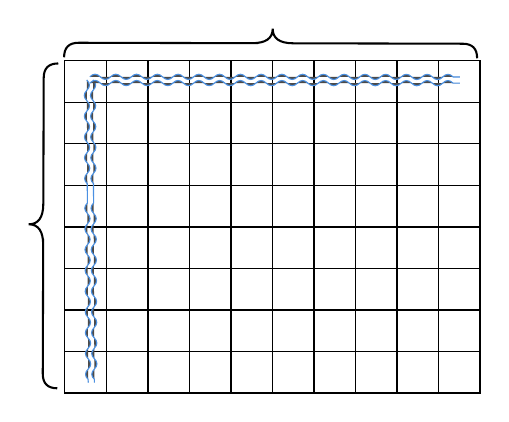
\begin{tikzpicture}[x=0.75pt,y=0.75pt,yscale=-1,xscale=1]
%uncomment if require: \path (0,300); %set diagram left start at 0, and has height of 300

%Shape: Brace [id:dp7713160444458687] 
\draw  [line width=0.75]  (428.9,72.4) .. controls (428.91,67.73) and (426.59,65.4) .. (421.92,65.39) -- (340.39,65.19) .. controls (333.72,65.17) and (330.4,62.83) .. (330.41,58.16) .. controls (330.4,62.83) and (327.06,65.15) .. (320.4,65.14)(323.4,65.14) -- (236.92,64.93) .. controls (232.25,64.92) and (229.91,67.25) .. (229.9,71.92) ;
%Shape: Grid [id:dp07818589413543853] 
\draw  [draw opacity=0][fill={rgb, 255:red, 255; green, 255; blue, 255 }  ,fill opacity=1 ] (230.31,73.67) -- (430.31,73.67) -- (430.31,233.67) -- (230.31,233.67) -- cycle ; \draw  [color={rgb, 255:red, 0; green, 0; blue, 0 }  ,draw opacity=1 ] (250.31,73.67) -- (250.31,233.67)(270.31,73.67) -- (270.31,233.67)(290.31,73.67) -- (290.31,233.67)(310.31,73.67) -- (310.31,233.67)(330.31,73.67) -- (330.31,233.67)(350.31,73.67) -- (350.31,233.67)(370.31,73.67) -- (370.31,233.67)(390.31,73.67) -- (390.31,233.67)(410.31,73.67) -- (410.31,233.67) ; \draw  [color={rgb, 255:red, 0; green, 0; blue, 0 }  ,draw opacity=1 ] (230.31,93.67) -- (430.31,93.67)(230.31,113.67) -- (430.31,113.67)(230.31,133.67) -- (430.31,133.67)(230.31,153.67) -- (430.31,153.67)(230.31,173.67) -- (430.31,173.67)(230.31,193.67) -- (430.31,193.67)(230.31,213.67) -- (430.31,213.67) ; \draw  [color={rgb, 255:red, 0; green, 0; blue, 0 }  ,draw opacity=1 ] (230.31,73.67) -- (430.31,73.67) -- (430.31,233.67) -- (230.31,233.67) -- cycle ;
%Straight Lines [id:da8818500948038484] 
\draw [color={rgb, 255:red, 74; green, 144; blue, 226 }  ,draw opacity=1 ][fill={rgb, 255:red, 74; green, 74; blue, 74 }  ,fill opacity=1 ]   (243.83,82.83) .. controls (245.51,84.48) and (245.52,86.15) .. (243.86,87.83) .. controls (242.2,89.5) and (242.21,91.17) .. (243.88,92.83) .. controls (245.55,94.49) and (245.56,96.16) .. (243.9,97.83) .. controls (242.25,99.5) and (242.26,101.17) .. (243.93,102.83) .. controls (245.6,104.49) and (245.61,106.16) .. (243.95,107.83) .. controls (242.29,109.5) and (242.3,111.17) .. (243.97,112.83) .. controls (245.64,114.49) and (245.65,116.16) .. (244,117.83) .. controls (242.34,119.5) and (242.35,121.17) .. (244.02,122.83) .. controls (245.69,124.49) and (245.7,126.16) .. (244.05,127.83) .. controls (242.39,129.5) and (242.4,131.17) .. (244.07,132.83) -- (244.09,137.14) -- (244.09,137.14) -- (244.11,142.14) .. controls (242.46,143.82) and (242.47,145.49) .. (244.14,147.14) .. controls (245.81,148.8) and (245.82,150.47) .. (244.16,152.14) .. controls (242.5,153.81) and (242.51,155.48) .. (244.18,157.14) .. controls (245.85,158.8) and (245.86,160.47) .. (244.21,162.14) .. controls (242.55,163.81) and (242.56,165.48) .. (244.23,167.14) .. controls (245.9,168.8) and (245.91,170.47) .. (244.26,172.14) .. controls (242.6,173.81) and (242.61,175.48) .. (244.28,177.14) .. controls (245.95,178.8) and (245.96,180.47) .. (244.3,182.14) .. controls (242.65,183.81) and (242.66,185.48) .. (244.33,187.14) .. controls (246,188.8) and (246.01,190.47) .. (244.35,192.14) .. controls (242.69,193.81) and (242.7,195.48) .. (244.37,197.14) .. controls (246.04,198.8) and (246.05,200.47) .. (244.4,202.14) .. controls (242.74,203.81) and (242.75,205.48) .. (244.42,207.14) .. controls (246.09,208.8) and (246.1,210.47) .. (244.44,212.14) .. controls (242.79,213.81) and (242.8,215.48) .. (244.47,217.14) .. controls (246.14,218.8) and (246.15,220.47) .. (244.49,222.14) .. controls (242.83,223.81) and (242.84,225.48) .. (244.51,227.14) -- (244.52,228.65) -- (244.52,228.65)(240.83,82.84) .. controls (242.51,84.5) and (242.52,86.17) .. (240.86,87.84) .. controls (239.2,89.51) and (239.21,91.18) .. (240.88,92.84) .. controls (242.55,94.5) and (242.56,96.17) .. (240.9,97.84) .. controls (239.25,99.51) and (239.26,101.18) .. (240.93,102.84) .. controls (242.6,104.5) and (242.61,106.17) .. (240.95,107.84) .. controls (239.3,109.51) and (239.31,111.18) .. (240.98,112.84) .. controls (242.65,114.5) and (242.66,116.17) .. (241,117.84) .. controls (239.34,119.51) and (239.35,121.18) .. (241.02,122.84) .. controls (242.69,124.5) and (242.7,126.17) .. (241.05,127.84) .. controls (239.39,129.51) and (239.4,131.18) .. (241.07,132.84) -- (241.09,137.16) -- (241.09,137.16) -- (241.11,142.16) .. controls (239.46,143.83) and (239.47,145.5) .. (241.14,147.16) .. controls (242.81,148.82) and (242.82,150.49) .. (241.16,152.16) .. controls (239.5,153.83) and (239.51,155.5) .. (241.18,157.16) .. controls (242.85,158.82) and (242.86,160.49) .. (241.21,162.16) .. controls (239.55,163.83) and (239.56,165.5) .. (241.23,167.16) .. controls (242.9,168.82) and (242.91,170.49) .. (241.26,172.16) .. controls (239.6,173.83) and (239.61,175.5) .. (241.28,177.16) .. controls (242.95,178.82) and (242.96,180.49) .. (241.3,182.16) .. controls (239.65,183.83) and (239.66,185.5) .. (241.33,187.16) .. controls (243,188.82) and (243.01,190.49) .. (241.35,192.16) .. controls (239.69,193.83) and (239.7,195.5) .. (241.37,197.16) .. controls (243.04,198.82) and (243.05,200.49) .. (241.4,202.16) .. controls (239.74,203.83) and (239.75,205.5) .. (241.42,207.16) .. controls (243.09,208.82) and (243.1,210.49) .. (241.44,212.16) .. controls (239.79,213.83) and (239.8,215.5) .. (241.47,217.16) .. controls (243.14,218.82) and (243.15,220.49) .. (241.49,222.16) .. controls (239.83,223.83) and (239.84,225.5) .. (241.51,227.16) -- (241.52,228.67) -- (241.52,228.67) ;
%Straight Lines [id:da2816175067396258] 
\draw [color={rgb, 255:red, 74; green, 144; blue, 226 }  ,draw opacity=1 ][fill={rgb, 255:red, 74; green, 74; blue, 74 }  ,fill opacity=1 ]   (242.33,81.33) .. controls (244,79.67) and (245.67,79.67) .. (247.33,81.34) .. controls (249,83.01) and (250.66,83.01) .. (252.33,81.34) .. controls (254,79.67) and (255.66,79.67) .. (257.33,81.34) .. controls (259,83.01) and (260.66,83.01) .. (262.33,81.34) .. controls (264,79.67) and (265.66,79.67) .. (267.33,81.34) .. controls (269,83.01) and (270.66,83.01) .. (272.33,81.34) .. controls (274,79.68) and (275.66,79.68) .. (277.33,81.35) .. controls (279,83.02) and (280.66,83.02) .. (282.33,81.35) .. controls (284,79.68) and (285.66,79.68) .. (287.33,81.35) .. controls (289,83.02) and (290.66,83.02) .. (292.33,81.35) .. controls (294,79.68) and (295.66,79.68) .. (297.33,81.35) .. controls (299,83.02) and (300.66,83.02) .. (302.33,81.36) .. controls (304,79.69) and (305.66,79.69) .. (307.33,81.36) .. controls (309,83.03) and (310.66,83.03) .. (312.33,81.36) .. controls (314,79.69) and (315.66,79.69) .. (317.33,81.36) .. controls (319,83.03) and (320.66,83.03) .. (322.33,81.36) .. controls (324,79.7) and (325.66,79.7) .. (327.33,81.37) .. controls (329,83.04) and (330.66,83.04) .. (332.33,81.37) .. controls (334,79.7) and (335.66,79.7) .. (337.33,81.37) .. controls (339,83.04) and (340.66,83.04) .. (342.33,81.37) .. controls (344,79.7) and (345.66,79.7) .. (347.33,81.37) .. controls (349,83.04) and (350.66,83.04) .. (352.33,81.38) .. controls (354,79.71) and (355.66,79.71) .. (357.33,81.38) .. controls (359,83.05) and (360.66,83.05) .. (362.33,81.38) .. controls (364,79.71) and (365.66,79.71) .. (367.33,81.38) .. controls (369,83.05) and (370.66,83.05) .. (372.33,81.38) .. controls (374,79.72) and (375.66,79.72) .. (377.33,81.39) .. controls (379,83.06) and (380.66,83.06) .. (382.33,81.39) .. controls (384,79.72) and (385.66,79.72) .. (387.33,81.39) .. controls (389,83.06) and (390.66,83.06) .. (392.33,81.39) .. controls (394,79.72) and (395.66,79.72) .. (397.33,81.39) .. controls (399,83.06) and (400.66,83.06) .. (402.33,81.4) .. controls (404,79.73) and (405.66,79.73) .. (407.33,81.4) .. controls (409,83.07) and (410.66,83.07) .. (412.33,81.4) .. controls (414,79.73) and (415.66,79.73) .. (417.33,81.4) -- (420.6,81.4) -- (420.6,81.4)(242.33,84.33) .. controls (244,82.67) and (245.66,82.67) .. (247.33,84.34) .. controls (249,86.01) and (250.66,86.01) .. (252.33,84.34) .. controls (254,82.67) and (255.66,82.67) .. (257.33,84.34) .. controls (259,86.01) and (260.66,86.01) .. (262.33,84.34) .. controls (264,82.67) and (265.66,82.67) .. (267.33,84.34) .. controls (269,86.01) and (270.66,86.01) .. (272.33,84.34) .. controls (274,82.68) and (275.66,82.68) .. (277.33,84.35) .. controls (279,86.02) and (280.66,86.02) .. (282.33,84.35) .. controls (284,82.68) and (285.66,82.68) .. (287.33,84.35) .. controls (289,86.02) and (290.66,86.02) .. (292.33,84.35) .. controls (294,82.68) and (295.66,82.68) .. (297.33,84.35) .. controls (299,86.02) and (300.66,86.02) .. (302.33,84.36) .. controls (304,82.69) and (305.66,82.69) .. (307.33,84.36) .. controls (309,86.03) and (310.66,86.03) .. (312.33,84.36) .. controls (314,82.69) and (315.66,82.69) .. (317.33,84.36) .. controls (319,86.03) and (320.66,86.03) .. (322.33,84.36) .. controls (324,82.7) and (325.66,82.7) .. (327.33,84.37) .. controls (329,86.04) and (330.66,86.04) .. (332.33,84.37) .. controls (334,82.7) and (335.66,82.7) .. (337.33,84.37) .. controls (339,86.04) and (340.66,86.04) .. (342.33,84.37) .. controls (344,82.7) and (345.66,82.7) .. (347.33,84.37) .. controls (349,86.04) and (350.66,86.04) .. (352.33,84.38) .. controls (354,82.71) and (355.66,82.71) .. (357.33,84.38) .. controls (359,86.05) and (360.66,86.05) .. (362.33,84.38) .. controls (364,82.71) and (365.66,82.71) .. (367.33,84.38) .. controls (369,86.05) and (370.66,86.05) .. (372.33,84.38) .. controls (374,82.72) and (375.66,82.72) .. (377.33,84.39) .. controls (379,86.06) and (380.66,86.06) .. (382.33,84.39) .. controls (384,82.72) and (385.66,82.72) .. (387.33,84.39) .. controls (389,86.06) and (390.66,86.06) .. (392.33,84.39) .. controls (394,82.72) and (395.66,82.72) .. (397.33,84.39) .. controls (399,86.06) and (400.66,86.06) .. (402.33,84.4) .. controls (404,82.73) and (405.66,82.73) .. (407.33,84.4) .. controls (409,86.07) and (410.66,86.07) .. (412.33,84.4) .. controls (414,82.73) and (415.66,82.73) .. (417.33,84.4) -- (420.6,84.4) -- (420.6,84.4) ;
%Shape: Brace [id:dp11340455600364296] 
\draw  [line width=0.75]  (227.1,74.9) .. controls (222.43,74.89) and (220.09,77.21) .. (220.08,81.88) -- (219.89,142.41) .. controls (219.87,149.08) and (217.53,152.4) .. (212.86,152.38) .. controls (217.53,152.4) and (219.85,155.74) .. (219.83,162.41)(219.84,159.41) -- (219.63,224.38) .. controls (219.62,229.05) and (221.94,231.39) .. (226.61,231.4) ;




\end{tikzpicture}

\end{figure}





% ------------------------------------------------------------------------------
% Reference and Cited Works
% ------------------------------------------------------------------------------

\bibliographystyle{IEEEtran}
\bibliography{References.bib}

% ------------------------------------------------------------------------------

\end{document}

% \adjustbox{margin=5pt}{\fbox {\sincfig{doppiaPrecisione}}} \\ 
